\documentclass[12pt,english]{article}
%\usepackage[margin=1in,footskip=0.25in]{geometry}

%\usepackage{helvet}
%\renewcommand{\familydefault}{\sfdefault}
\renewcommand\refname{\vskip -1cm}
%\renewcommand{\rmdefault}{phv} % Arial
%\renewcommand{\sfdefault}{phv} % Arial
\usepackage{setspace}
\usepackage{wrapfig}
\usepackage{amsmath}
\usepackage{amssymb}
\usepackage{graphicx}
\usepackage{mathrsfs}
\usepackage{bm}
\usepackage{wasysym}
\usepackage{placeins}
\usepackage{multirow}
\usepackage[T1]{fontenc}
\usepackage[authoryear]{natbib}

%\usepackage[style=authoryear,sorting=ynt]{biblatex}

\usepackage{framed}
\usepackage{caption}
\usepackage{longtable}
\usepackage{geometry}
\usepackage{lineno}

\geometry{verbose,letterpaper,tmargin=2.54cm,bmargin=2.54cm,lmargin=2.54cm,rmargin=2.54cm}


\begin{document}
\begin{spacing}{1.9}


\title{The effect of starvation on the dynamics of consumer populations}
\author{Yeakel, Kempes, \& Redner}
\maketitle

\linenumbers
%\begin{flushleft}


%Focus on the tradeoff between REPRODUCTION AND SURVIVAL AS A FUNCTION OF ENERGETIC STATE

The behavioral ecology of most, if not all, organisms is influenced by the energetic state of individuals.
An individual's energetic state directly influences how it invests its stores in an uncertain environment.
Such behaviors are generally manifested as trade-offs, which often concern investing in individual maintenance and growth (somatic effort) or allocating energy towards reproduction (reproductive effort) \citep{Martin:1987dl,Kirk:1997cc,Kempes:2012hy}. %among a host of other behavioral duties [REFS].
The timing of these behaviors is often important and is under strong selective pressure, as they tend to have large effects on the future fitness of the organism \citep{Mangel:1988uaa}.
%For example, rotifers that reproduce have lower survival rates than those that don't when they are under nutritional stress.
To what extent, and when, organisms invest in somatic vs. reproductive expenditures may be driven by habitat, seasonality, evolutionary history, inter- or intra-specific interactions, as well as resource limitation.
Importantly, the influence of resource limitation on an organism's ability to maintain its nutritional stores may lead to repeated delays or shifts in reproduction over the course of an organism's life. %and the subsequent loss of nutritional reserves
%Such tradeoffs are also bound to have population-level consequences, although this has received little theoretical or empirical attention.

%The reproductive vs. storage tradeoff
Maximizing fitness between growth and maintenance activities vs. reproductive efforts in large part structures the life-history of species, and this can be achieved by alternative behavioral strategies or via physiological switches, both of which are sensitive to resource availability.
%Reproduction can be separated from somatic growth/maintenance by a variety of potential mechanisms:
%Multiple mechanisms contribute to the differentiation of these behaviors:
Behavioral changes in somatic or reproductive investment occur in response to limited resources \citep{Morris:1987eo}.
%, while stress can generally lead to reprodusuppression of reproductive behaviors \citep{Morgan:1999do}. 
For example, reindeer invest less in calves born after harsh winters (when the mother's energetic state is poor) than in calves born after moderate winters \citep{Tveraa:2003fq}, whereas many bird species invest differently in broods during periods of resource scarcity \citep{Daan:1988va,Jacot:2009dv}, sometimes delaying or foregoing reproduction for a breeding season \citep{Martin:1987dl,Barboza:2002in}.
Such breeding behaviors is generally referred to as \emph{capital breeding}
%Resource limitation can also alter the behaviors of species in well-mixed environments: 
Freshwater and marine zooplankton have been observed to avoid reproduction under nutritional stress \citep{Threlkeld:1976ih}, with those that do reproduce evincing lower survival rates \citep{Kirk:1997cc}, while artificially induced stress has been observed to decrease reproductive success in Atlantic cod \citep{Morgan:1999do}.
Organisms may also separate maintenance and growth from reproduction over space and time. 
Many salmonids, birds, and some mammals return to migratory breeding sites to reproduce after one or multiple seasons in alternative environments spent accumulating body mass and nutritional reserves \citep{Weber:1998jg,Mduma:1999cp,Moore:2014hi}.


Physiological mechanisms also play an important role in regulating reproductive expenditures during periods of high-risk.
Diverse mammals (47 species in 10 families) exhibit delayed implantation whereby females postpone fetal development (blastocyst implantation) to time with accumulation of nutritional reserves \citep{Mead:1989dt,Sandell:1990kw}. %, including multiple species of Grizzly bears (\emph{Ursus horribilis}) and the European badger (\emph{Meles melesc}) \citep{Woodroffe:1995id
Furthermore, many mammals (including humans) suffer irregular menstrual cycling and higher abortion rates during periods of nutritional stress \citep{Bulik:1999eo,Trites:2003cc}.
In the extreme case of unicellular organisms, nutrition is unavoidably linked to reproduction because the nutritional state of the individual regulates all aspects of the cell cycle \citep{Glazier:2009hq}.
%great tits invest more energy into broods when resource abundance is greater, while food availability is generally seen to correlate with clutch size among many bird species \citep{Daan:1988va}.
%The mechanisms that control reproductive effort as a function of energetic reserves differ among species.
%Even humans alter their growth trajectories and have higher chances of fetal abortion during periods of starvation.
%Thus, some organisms partition reproductive vs. foraging effort over both space and time, whereas other rely on physiological mechanisms to optimize reproductive success against survival when adequate resources are unavailable.
The existence of so many independently evolved mechanisms across such a diverse suite of organisms points to the importance and universality of the fundamental tradeoff between somatic and reproductive investment, however the dynamic implications of these constraints are unknown.

%To population-level effects
The mechanisms by which different organisms avoid or delay reproduction during times of nutritional stress has received tremendous empirical and theoretical attention owing to the importance of these activities in shaping life-history \citep{Cody:1966fk,Martin:1987dl,Mangel:1988uaa}.
Less well understood is how resource limitation and these behavioral/physiological tradeoffs affect dynamics at the level of the population.
% when organisms are able to avoid the risk of spending energy on reproduction when starvation is likely.
Traditional Lotka-Volterra models assume a dependence of consumer population growth rates on resource density, thus \emph{implicitly} incorporating the requirement of resource availability for reproduction \citep{murdoch:2003}.
Although this implicit dependence connects resource limitation to lower consumer growth rates, the following biological realities are not included: 
\emph{i}) some individuals experience nutritional stress at a given time and under a given set of external conditions, while others do not; those that do have multiple pathways enabling reproductive cessation; 
\emph{ii}) the portion of the population that is not nutritionally stressed is expected to reproduce at a near-constant rate and this is -- averaged across species -- determined strongly by body size \citep{Kempes:2012hy};
\emph{iii}) the rates that individuals transition from nutritionally poor to replete states and back have different metabolically-constrained timescales that can lead to reproductive lags.
Importantly, the exclusion of these biological details may have important dynamic shortcomings, masking the effects of starvation on consumer population dynamics.


Resource limitation and the subsequent effects of starvation may be alternatively accounted for \emph{explicitly}, such that reproduction is permitted only for individuals with sufficient energetic reserves.
Though straightforward conceptually, incorporating the energetic dynamics of individuals \citep{Kooi2000} into a population-level framework \citep{Kooi2000,Sousa:2010ez} presents numerous mathematical obstacles \citep[in particular a lack of smoothness, or differentiability;][]{Diekmann:2010da}, and often suffers from over-fitting due to an overabundance of parameters.
These issue have limited the development of theoretical models that may aid our understanding of the effects of such tradeoffs on population dynamics.
An alternative approach to individual-to-population frameworks is redirecting focus to macroscale relationships guiding somatic vs. reproductive investment in a consumer-resource system.

%[Here we use body size and allometries to capture a wide variety of taxonomic diversity]
%[There isn't a deep understanding with how models vary across different life histories, traits, etc... how do equations change with allometric constraints for different class of organisms? 
%i.e. Use body size as a generating parameter to capture a wide variety of diversity.]

%What we did...
Here we explore how the energetic tradeoff between maintaining and building somatic tissue vs. reproduction can influence the dynamics of populations, and how such dynamics may be determined by allometric constraints.
We begin by establishing a simple Nutritional State-structured population Model (NSM), where consumer starvation, and cessation of reproduction, is the consequence of resource limitation.
Similarly, recovery from the starved to a reproductive state increases with resource density.
%that captures the essential dynamics of energetic vs. reproductive tradeoffs
%and explore the impact of different fluxes on system-level stability.
Importantly, the rate at which consumers decline and recover from a starved state is wholly constrained by metabolism.
By relating different rate constants to allometric constraints, we uncover important relationships between the timescales of physiological and reproductive processes, and show how organisms of different body sizes and taxonomic affinities may be prone to alternative dynamics.

%By deriving allometric constraints for the starvation, recovery, and reproductive timescales of the consumer-resource system, 
We show that rates of starvation and recovery tend to result in systems with stable, non-cyclic fixed points and that the ratio between the rate of starvation and recovery may -- in part -- contribute to lower size limitations.
Moreover, larger consumer body size results in rates that are less prone to cyclic dynamics than are rates for smaller organisms, pointing to potential empirical verification of the NSM framework.
Finally, we show that rates of starvation and recovery appear to be constrained to a parameter range where both transient and equilibrial population dynamics result in the lowest risk of extinction for the consumer.
This surprising result suggests that the risks associated with different fluxes of consumers in and out of a starved (non-reproductive) state may serve as an important selective driver over evolutionary time.




\noindent {\bf Starvation dynamics} \\ \nonumber
We integrate the somatic/reproductive tradeoff into the dynamics of a consumer-resource system by dividing the consumer population into discrete energetic states, the occupation of each being contingent on the consumption of a single resource $R$.
In the NSM there are only two energetic states for the consumer population: \emph{i}) an energetically replete (full) state $F$, where the consumer reproduces at a constant rate $\lambda$, and \emph{ii}) an energetically deficient (hungry) state $H$, where reproduction is suppressed, and mortality occurs at rate $\mu$.
Consumers transition from state $F$ to state $H$ by starvation at rate $\sigma$ and in proportion to the lack of resources $(1-R)$.
Conversely, consumers recover from state $H$ to the full state $F$ at rate $\rho$ and in proportion to $R$.
The resource has logistic growth with a linear growth rate $\alpha$ and a carrying capacity of unity.
Resources are eliminated by the consumer in both states: by energetically deficient consumers at rate $\rho$, and by energetically replete consumers at rate $\beta$.
Accordingly, the system of equations is written


\begin{align}
\begin{split}
\dot{F} &= \lambda F + \rho RH - \sigma (1-R)F,  \\
\dot{H} &= \sigma (1-R)F - \rho RH - \mu H,  \\
\dot{R} &= \alpha R(1-R) - R(\rho H+ \beta F).
\label{eq_specific}
\end{split}
\end{align}

%[NSM = Nutritional State Model]
%[LVM = Lotka Volterra Model]


There are three steady states for the NSM: two trivial fixed points at $(R^*=0,H^*=0,F^*=0)$ and $(R^*=1,H^*=0,F^*=0)$, and one non-trivial internal fixed point at

\begin{align}
\begin{split}
F^* &= \frac{\alpha  \lambda  \mu  (\mu +\rho )}{(\lambda  \rho +\mu  \sigma ) (\lambda  \rho +\mu  \beta)}, \\
H^* &= \frac{\alpha  \lambda ^2 (\mu +\rho )}{(\lambda  \rho +\mu  \sigma ) (\lambda  \rho +\mu  \beta)}, \\
R^* &= \frac{\mu  (\sigma -\lambda )}{\lambda  \rho +\mu  \sigma }.
\end{split}
\end{align}

\noindent Because there is only one internal fixed point, as long as it is stable the population trajectories will serve as a global attractor for any set of positive initial conditions.
%Analysis of the stability of the NSM is explored with respect to the local stability of the internal steady state, which is the only feasible steady state as long as both the consumer and resource have non-zero, positive, values.
In a multidimensional system, linear stability is determined with respect to the Jacobian Matrix $\bf J|_*$ (where $|_*$ denotes evaluation at the internal steady state), where each element of the matrix is defined by the partial derivative of each differential equation with respect to each variable.
%In the case of the 2-stage consumer model, the Jacobian evaluated at the internal steady state (denoted by $|_*$) is written
%
%\begin{equation}
%\mathbf{J}|_* =
%%\left(
%%\begin{array}{ccc}
%% -F^* m+(1-R^*) a -R^* a -H^* \rho  & -R^* \rho  & -m R^* \\
%% -H^* \rho -F^* \sigma  & -\mu -R^* \rho  & (1-R^*) \sigma  \\
%% H^* \rho +F^* \sigma  & R^* \rho  & \lambda -(1-R^*) \sigma  \\
%%\end{array}
%%\right).
%\left(
%\begin{array}{ccc}
% -\frac{\lambda  \rho  (\sigma - \lambda )}{\lambda  \rho +\mu  \sigma } & \frac{\mu  \rho  (\sigma -\lambda )}{\lambda  \rho +\mu  \sigma } & \frac{\alpha  \lambda  (\mu +\rho )}{m \mu +\lambda  \rho } \\
% \frac{\lambda  (\mu +\rho ) \sigma }{\lambda  \rho +\mu  \sigma } & -\frac{\mu  (\mu +\rho ) \sigma }{\lambda  \rho +\mu  \sigma } & -\frac{\alpha  \lambda  (\mu +\rho )}{m \mu +\lambda  \rho } \\
% -\frac{m \mu  (\sigma - \lambda)}{\lambda  \rho +\mu  \sigma } & -\frac{\mu  \rho  (\sigma - \lambda )}{\lambda  \rho +\mu  \sigma } & -\frac{\alpha  \mu  (\sigma - \lambda)}{\lambda  \rho +\mu  \sigma } \\
%\end{array}
%\right).
%\end{equation}


%Transcritical bifurcation
If the parameters of $\bf J|_*$ are such that the real part of its leading eigenvalue is $<0$, then the system is stable to small pulse perturbations. 
In the case of the NSM, stability is conditioned on the consumer's starvation rate $\sigma$ relative to the its reproduction rate $\lambda$.
As $\sigma$ becomes less than $\lambda$, the $R^*$ crosses the origin and the fixed point becomes unstable.
This condition $\sigma = \lambda$  marks a transcritical (TC) bifurcation, thus marking a hard boundary below which the system becomes unphysical due to the unregulated growth of the consumer population.
That the timescale of reproduction is larger than the timescale of starvation is intuitive for macroscopic organisms, as the rate at which one loses tissue due to lack of resources is generally much faster than reproduction, though we will show using allometric principles that this relationship always holds.
%such that if a consumer's starvation rate is lower than it's reproductive rate, the consumer population's growth becomes exponential and unphysical.
%Thus, the timescale of starvation must be less than the timescale of reproduction, an expectation that will hold for most classes of organisms, which we will show by deriving allometric scaling relationship that serve to constrain the covariation of parameter values.
%[Explain what a transcritical bifurcation means in terms of the dynamics. From a regime where resources are negative and consumer populations become infinite to one that is biological feasable]
%As such, a transcritical bifurcation exists at $\lambda = \sigma$, such that the existence of an internal stable fixed point is dependent on the condition that $\sigma > \lambda$.
%This means that the rate of starvation must be greater (operating on a smaller timescale) than the rate of consumer reproduction (operating on a relatively longer timescale).
%This general expectation will hold for most classes of organisms, which we will show by deriving allometric scaling relationship that serve to constrain the covariation of parameter values.
% while the exact difference in timescales between reproduction and starvation can be derived using allometric scaling relationships.
%Kempes (REF) has shown that population growth rates scale to $M^{\alpha-1}$ (where $M$ is the reproductive mass of an organism and $\alpha$ is the scaling exponent), whereas starvation is necessarily bound to shorter timescales, which will be elaborated on below.


%Hopf bifurcation
In addition to the hard bound defined by the TC bifurcation, oscillating or cyclic dynamics present an implicit constraint to persistence by increasing the risk of extinction.
%also present certain constraints to the feasibility of populations.
%Oscillating, or cyclic, dynamics present additional risks to populations.
If cycles are large, stochastic effects may result in either the consumer or resource population.
In continuous-time systems, a stable limit cycle arises when a pair of complex conjugate eigenvalues crosses the imaginary axis to attain positive real parts \citep{GuckHolmes}.
%Of additional interest is the existence of parameter regions that permit the existence of oscillatory, or cyclic, dynamics.
This condition is called a Hopf bifurcation, and is defined by ${\rm Det}({\bf S}) = 0$, where $\bf S$ is the Sylvester matrix, which is composed of the coefficients of the characteristic polynomial describing the Jacobian \citep{Gross:2004p2428}.
In addition to the onset of stable cycles, as a system with a stable fixed point nears the Hopf bifurcation, transient or decaying cycles can grow in magnitude.
Given that ecological systems exist in a state of constant perturbation \citep{Hastings:2001jh}, even the onset of transient cycles that decay over time can increase the risk of extinction \citep{Neubert:1997wk,Caswell:2005eo,Neubert:2009td}, such that the distance of a system from the Hopf bifurcation, even in the stable region, is relevant to persistence.

%Although the Hopf condition for the specific 2-stage model cannot be easily written, the analytical solution can be explored using a symbolic computational language such as \emph{Mathematica}.





\noindent {\bf Allometric constraints} \\ \nonumber
%[Link Allometry stuff to our model - what does it provide to the story]
%[Introduce biological and linked constraints]
%[Allometries capture vast amounts of diversity via a single parameter --- body size]
%[Allometries have captured intterest etc across multiple scales and biological classes of organisms]
Chris - Linking paragraph here -- what does allometry provide to the story? Biological, linked constraints... vast amounts of diversity in a small number of parameters. Etc.



%Second paragraph
Nearly all of the rates described in the NSM are to some extent governed by consumer metabolism, and thus can be estimated based on known allometric constraints. 
The scaling relationship between an organism's metabolic rate $B$ and its body size at reproductive maturity $M$ is well documented \citep{West:2002it} and plays a central role in a variety of scaling relationships.
Organismal metabolic rate $B$ is known to scale as $B = B_0 M^\eta$, where $\eta$ is the scaling exponent, generally assumed to be $3/4$ for metazoans, and varies in unicellular species between $\eta\approx 1$ in eukaryotes and $\eta\approx 1.76$ in bacteria \citep{DeLong:2010dy}. Several efforts have shown how a partitioning of this metabolic rate between growth and maintenance purposes can be used to derive a general equation for the growth trajectories and growth rates of organisms ranging from bacteria to metazoans \citep{Kempes:2012hy}. More specifically, the interspecific trends in growth rate can be approximated by $\lambda = \lambda_0 M^{\eta-1}$. This relationship is derived from the simple balance
 \begin{equation}
 B_{0}m^{\eta}=E_{m}\frac{dm}{dt}+B_{m}m
 \label{balance}
 \end{equation}
 [a and b notation --- these parameters are easily measured bioenergetic parameters which are often approximately invariant across organisms of vastly different size. Our notation seeks to illustrate that the allometric model fundamentally depends on a small number of free parameters.]
 where $E_{m}$ is the energy needed to synthesize a unit of mass, $B_{m}$ is the metabolic rate to support an existing unit of mass, and $m$ is the mass at any point in development. It is useful to explicitly write this balance because it can also be modified to understand the rates of both starvation and recovery from starvation. [Spell out the connection to nutritional state more explicitly] [As we will see it is possible to derive both sigma and rho from this balance]
 
For the rate of starvation, we make the simple assumption that an organism must meet its maintenance requirements using digested mass as the sole energy source. This assumption implies the simple metabolic balance 
\begin{equation}
\frac{dm}{dt}E_{m}^{\prime}=-B_{m}m
\end{equation}
where $E_{m}^{\prime}$ is the amount of energy stored in a unit of existing body mass which may differ from  $E_{m}$, the energy required to synthesis a unit of biomass. Give the adult mass, $M$, of an organism this energy balance prescribes the mass trajectory of a starving organism:
\begin{equation}
m\left(t\right)=Me^{-B_{m}t/E_{m}^{\prime}}.
\end{equation}
Considering that only certain tissues can be digested for energy, for example the brain cannot be degraded to fuel metabolism, we define the rate for starvation and death by the timescales required to reach specific fractions of normal adult mass. We define $m_{starve}=\epsilon M$ where it could be the case that organisms have a systematic size-dependent requirement for essential tissues, such as the minimal bone or brain mass. For example, considering the observation that body fat in mammals scales with overall body size according to $M_{f}=f_{0}M^{\gamma}$, and assuming that once this mass is fully digested the organism begins to starve, would imply that $\epsilon=1-f_{0}M^{\gamma}/M$. Taken together the time scale for starvation is given by
\begin{equation}
t_{\sigma}=-\frac{E_{m}\log\left(\epsilon\right)}{B_{m}}.
\end{equation}
The starvation rate is $\sigma=1/t_{\sigma}$, which implies that $\sigma$ is independent of adult mass if $\epsilon$ is a constant, and if $\epsilon$ does scale with mass, then $\sigma$ will have a factor of $1/\log\left(1-f_{0}M^{\gamma}/M\right)$. In either case $\sigma$ does not have a simple scaling with $\lambda$ which is important for the dynamics that we later discuss. 

The time to death should follow a similar relationship, but defined by a lower fraction of adult mass, $m_{death}=\epsilon^{\prime} M$. Consider, for example, that an organism dies once it has digested all fat and muscle tissues, and that muscle tissue scales with body mass according to $M_{mm}=mm_{0}M^{\zeta}$, then $\epsilon^{\prime}=1-\left(f_{0}M^{\gamma}+mm_{0}M^{\zeta}\right)/M$. Muscle mass has been shown to be roughly proportional to body mass \cite{muscle} in mammals and thus  $\epsilon^{\prime}$ is effectively $\epsilon$ minus a constant. Thus
\begin{equation}
t_{\mu}=-\frac{E_{m}\log\left(\epsilon^{\prime}\right)}{B_{m}}
\end{equation}
and $\mu=1/t_{\mu}$. 

It should be noted that we have thus far used mammalian allometry to describe the size-based relationships for growth, starvation, and death. However, our presentation is general, and other functional forms for $\epsilon$, for example, could be determined for other classes of organisms. Considering bacteria, we might expect that starvation or death is defined by the complete digestion of proteins, and in Table \ref{parameter-values} we provide all parameter values for bacteria which we later use as a comparison in our analysis. 

The rate of recovery $\rho = 1/t_\rho$ requires that an organism accrues tissue from the starving state to the full state.
We again use the balance given in Equation \ref{balance} to find the timescale to return to the mature mass from a given reduced starvation mass. The general solution to Equation \ref{balance} is given by
\begin{equation}
m\left(t\right)=\left[1-\left(1-\frac{b}{a}m_{0}^{1-\alpha}\right)e^{-b\left(1-\alpha\right)t}\right]^{1/\left(1-\alpha\right)}\left(\frac{a}{b}\right)^{1/\left(1-\alpha\right)}
\end{equation}
with $a=B_{0}/E_{m}$ and $b=B_{m}/E_{m}$. We are then interested in the timescale, $t_{\rho}=t_{2}-t_{1}$, which is the time it takes to go from $m\left(t_{1}\right)=\epsilon M$ to $m\left(t_{2}\right)=M$, which has the final form of 
\begin{equation}
t_{\rho}=\frac{\log \left(1-\left(M \left(\frac{a}{b}\right)^{\frac{1}{\alpha -1}}\right)^{1-\alpha }\right)-\log \left(1-\left(M \epsilon  \left(\frac{a}{b}\right)^{\frac{1}{\alpha
   -1}}\right)^{1-\alpha }\right)}{(\alpha -1) b}.
\end{equation}




%Population growth requires that individuals 


%\begin{align}
%\lamdba &=  \nonumber \\
%\sigma &= \nonumber \\	
%\end{align}


\noindent {\bf The stabilizing effects of allometric constraints} \\ \noindent
Although starvation leads to mortality risk for the individual, a moderate amount promotes persistence of both consumer and resource populations.
%Sigma and rho vs. Hopf and TC
Analysis of the NSM shows that (non-cyclic) stability of the fixed point generally requires a higher starvation rate $\sigma$ relative to the recovery rate $\rho$.
The intuition behind this is that transition to the hungry (non-reproductive) state permits the resource to recover and transient dynamics to subside, whereas a low $\sigma$ overloads the system with energetically-replete (reproducing) individuals, thus producing maintained oscillations between consumer and resource (Fig. \ref{Hopfb}).
However if $\sigma$ is too large, mortality due to starvation depletes the consumer population, resulting in a lower steady state density, and an opposingly higher steady state density for the resource.

Whereas the rate of consumer growth defines a hard bound of biological feasibility (the TC bifurcation), the rate of starvation determines the sensitivity of the consumer population to changes in resource density.
While higher rates of starvation result in lower steady state population size -- increasing the risk of stochastic extinction -- lower rates of starvation result in a system poised near either the TC or Hopf bifurcation (or both), which will lead to extinction of the resource or the development of cyclic oscillations, respectively.
Which bifurcation is approached is wholly dependent on the rate of recovery: if it is high, then cyclic dynamics will develop; if it is low, resource extinction becomes more likely.




%Bifurcation space as a function of mass
As the allometric derivations of NSM rate laws reveal, $\sigma$ and $\rho$ are not independent parameters, such that the bifurcation space shown in Fig. \ref{Hopfb} cannot be freely navigated if assuming biologically reasonable parameterizations.
Given the parameterization for mammals shown in Table \ref{xx} with mass $M$ as the only free parameter, rates of starvation and recovery are constrained to a fairly small window of potential values.
Importantly, for larger organismal masses, the distance between $\sigma(M)$ and $\rho(M)$ compared to both the TC and Hopf bifurcations is increased.
Uncertainty in allometric parameters (20\% variation around the mean; Fig. \ref{xx}) results in little difference in the position of both bifurcations as well as consumer energetic rates.
This suggests 
1)that small mammals are more prone to population oscillations -- including both stable limit cycles as well as transient cycles -- than large mammals, and
2) the decreasing distance to the Hopf bifurcation with lower body sizes is suggestive of a dynamic barrier to the mass of endothermic organisms.
Although the prediction of oscillations with smaller body sizes  generally holds, empirical observations of large animal population cycles are plagued by long generation times and the influence of top-down effects [REFS].

%Effect noise

%NOTES 7/8/16
%Calder has a hypothesis that period ~ Mass^(1/4).
%Can we get "transient period" from Jacobian?
%Lots of food web lit on stabilizing effects of body size! Brose, Petchey for instance. Good for discussion.



both the location of TC and Hopf bifurcations over $\sigma$ and $\rho$ relative to the allometrically-determined starvation and recovery rates of species across different body sizes 
%Mass changes the values of the fixed points as well

[First describe the dynamics of the model and HOW IT WORKS]
[Then Allometry and stability]

Analysis of the 2-stage consumer resource model shows that the equilibrial states of both populations are highly sensitive to changes in  starvation and recovery rates of the consumer.
The consumer and resource population densities vary inversely: when the consumer densities are high, resource densities are low, and vice versa.
High starvation and low recovery rates result in low consumer densities and high resource densities. %whereas the opposite is true for low starvation and high recovery rates.
If starvation rates are low, resources have a fixed point near zero for any value of the recovery rate.
Full and hungry consumer stages tend have fixed points that are tightly correlated, the extent to which is driven by the similarity of consumer growth and mortality rates; if $\lambda = \mu$, then $F^* = H^*$.

%Transcritical & rate law ranges
A transcritical bifurcation exists at $\lambda = \sigma$, such that the condition $\sigma > \lambda$ is required for biologically reasonable dynamics.
The TC bifurcation occurs in this model because we have assumed that the portion of the population that is not starved reproduces at a constant rate.
Because the process of starvation is incorporated explicitly, the consumer's rate of reproduction is not dependent on the density of resources.
In fact, the existence of the TC bifurcation at $\lambda = \sigma$ reveals an important biological insight. 
Reproduction requires maintenance and growth of biological tissues, both of which have strong scaling relationships with body size.
Recent work by Kempes et al. [REF] derived the timescale of reproduction in terms of allometric considerations, where $t_\lambda \propto M^{1-\eta}$ (REF).
Starvation is the loss of energy required for maintenance, and we have shown it to have a timescale $t_\sigma \propto \log(M)$.
Accordingly, the timescale of reproduction is always larger than the timescale of starvation, such that $\lambda$ must be less than $\sigma$ by definition.
A third important parameter in our framework is the rate of recovery.
The recovery timescale $t_\rho$ controls the rate at which individuals move from the hungry class to the full class, and this requires not only tissue maintenance, but growth, such that it is bounded on the short side by $t_\sigma$.
Moreover, [why is recovery timescale bounded on the high side], such that it is bounded on the long side by $t_\lambda$.
Thus, incorporating allometric considerations shows us that $\lambda < \rho < \sigma$ (alternatively $t_\lambda > t_\rho > t_\sigma$).

%Hopf bifurcation and oscillations sigma vs. rho
The 2-stage consumer resource model exhibits two qualitatively different behavioral regimes.
Because portions of the consumer population exist in either full or hungry states simultaneously, the internal fixed point can either be a stable equilibrium, or exhibit sustained oscillatory behavior, depending on the rates of starvation $\sigma$ and recovery $\rho$.
The transition from stable non-oscillatory dynamics to oscillatory dynamics occurs at the Hopf bifurcation condition where two complex conjugate eigenvalues cross the imaginary axis and attain positive real parts.
Although there is an analytical solution to the Hopf bifurcation condition, it cannot be written efficiently.

When the starvation rate is low, oscillatory dynamics are more likely to occur for a given value of the recovery rate.
This can be understood intuitively: for low starvation rates, resources are depressed by an infusion of full consumers, which subsequently starve thereby allowing the resource to recover and continuing the cycle.
When the starvation rate is high, the response of consumer growth to resource abundance is muted, such that oscillations tend to decay over time.
Thus, higher starvation rates $\sigma$ desensitizes changes in the consumer population to changes in resource density, and lower rates of recovery $\rho$ amplifies this effect.

%Hopf bifurcation as a function of b
Both full and hungry consumers remove resources at rates $b$ and $\rho$, respectively.
As the rate of resource consumption by full consumers increases, the Hopf condition changes from a convex to a concave function over $\sigma$, limiting the potential for oscillatory dynamics.
These rates are considered separately because full consumers need only to maintain their tissues, whereas hungry consumers require both growth and maintenance, such that $t_\rho > t_b$, or $\rho < b$.
If this constraint is enacted, the likelihood of oscillatory dynamics is reduced for a given 



If instead the consumer's growth was proportional to resource abundance, such that the effects of starvation on reproduction were incorporated explicitly (where the 2-stage consumer resource model collapses to the Lotka-Volterra consumer-resource model with logistic growth of the resource), the TC bifurcation exists only for $\lambda = \mu$, such that the rate of mortality cannot exceed the intrinsic birth rate.


 whereas the traditional Lotka-Volterra dynamic assumes that the reproductive rate of the consumer is scaled to resource density, such that the growth function would be $G(F,R) = \lambda R F$.
Thus, the Lotka-Volterra dynamic \emph{implicitly} accounts for starvation in reducing the reproductive rate of the consumer.
However, our 2-stage model \emph{explicitly} accounts for starvation as well as recovery, such that individuals who are not starved should adopt a reproductive rate independent of resource density.



We have used scaling relationships between tissue turnover and growth to strictly constrain 5/6 population-level parameters in our 2-stage consumer resource model (including the mortality rate $t_\mu$, which we have shown is just a xxx of $t_\sigma$).
This exercise accomplishes two goals:
1) it allows us to constrain the plausible parameter space of the two-stage model, and 
2) 

This allows us to derive many aspects of the system in terms of consumer body mass $M$ and the allometric scaling exponent $\eta$.



\noindent {\bf Minimizing extinction risk} \\ \nonumber






%
%
%%Starving Random Walk
%In our modeling, foragers look for food by wandering in this changing
%environment.  If such a search is successful, the forager is satiated and it
%can engage in the essential activity of reproduction.  However, if the search
%is unsuccessful for a sufficiently long period, the forager ``starves''.
%Such a forager can do nothing else but forage, until it either finds food and
%again becomes satiated or it dies when it goes too long without finding
%nourishment.  These rules are reminiscent of the ``starving random walk''
%model, where a single random walk can take $\mathcal{S}$ steps without
%encountering food before starving to death.  Moreover, the resource does not
%regenerate, so that the forager ultimately starves to death.  For this
%idealized model, it was found that the average lifetime of the forager scales
%algebraically with $\mathcal{S}$ in $d\!=\!1$ and $d\!=\!2$ dimensions, and
%as $\exp(-A\mathcal{S}^\omega)$ for $d>2$.  Here the exponent
%$\omega\approx \frac{1}{2}$ for $d=3$, while $\omega\to 1$ only as
%$d\to \infty$, with the latter behavior corresponding to the mean-field
%limit.  As we will discuss, regeneration of the resource, together with the
%behavioral change between starving and satiated foragers leads to still much
%richer dynamical behavior.



%The reproductive tradeoff as a strategy
%
\clearpage

\begin{table}[h]
\caption{Parameter Values For Various Classes of Organisms}
\label{parameter-values}
    \begin{center}
    \small
     \begin{tabular}{| p{1.2cm}| p{3.2cm} | p{2.6cm} | p{3.2cm} | }
     \hline
     & {\bf Mammals} & {\bf Unicellular Eukaryotes} & {\bf Bacteria} \\
     \hline
   $\eta$ & $3/4$ & & $1.70$ \\ 
   $E_{m}$ & $10695$ (J gram$^{-1}$) & & $10695$ (J gram$^{-1}$) \\ 
   $E_{m}^{\prime}$ & $\approx E_{m}$ & & $\approx E_{m}$ \\ 
   $B_{0}$ & $0.019$ (W gram$^{-\alpha}$) & & $1.96\times10^{17}$ \\
   $B_{m}$ & $0.025$ (W gram$^{-1}$)   & & $0.025$ (W gram$^{-1}$)\\
   $a$ & $1.78\times10^{-6}$ & & $1.83\times10^{13}$ \\ 
   $b$ & $2.29\times10^{-6}$ & & $2.29\times10^{-6}$ \\  
   $\eta-1$ & $-0.21$ & & $0.73$ \\ 
   $\lambda_{0}$ & $3.39\times10^{-7}$ (s$^{-1}$ gram$^{1-\eta}$) & & $56493$ \\ 
   $\gamma$ & $1.19$ & & $0.68$ \\ 
   $f_{0}$ & $0.02$ & & $1.30\times10^{-5}$ \\ 
   $\zeta$ & $1.01$ & & \\ 
   $mm_{0}$ & $0.32$ & & \\ 
   
      
   \hline
    \end{tabular}
    \end{center}
   \end{table}

\clearpage


 \begin{figure}[h]
 	\centering
 	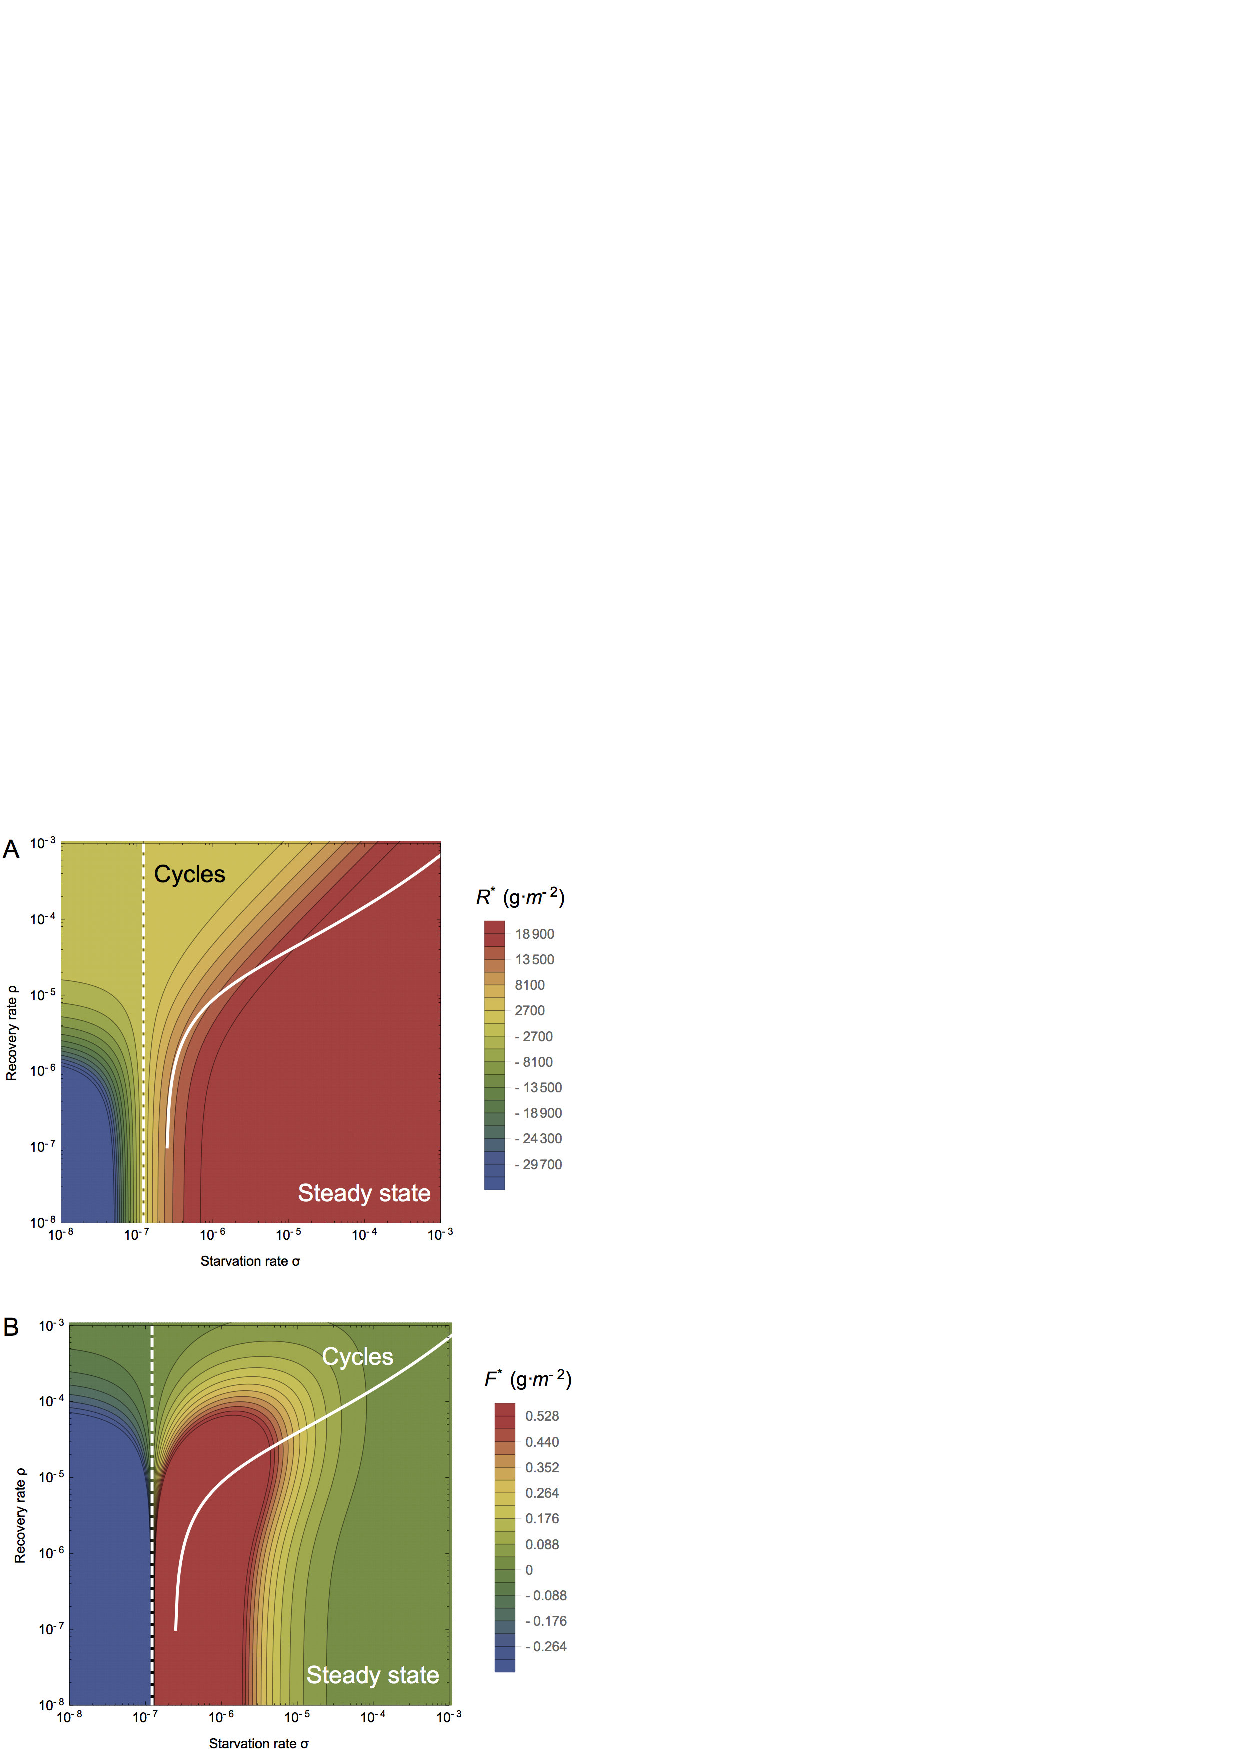
\includegraphics[width=0.75\textwidth]{fig_FixedPoint.pdf}
 	\caption{
 	}
 	\label{Hopfb}
 \end{figure}


 \begin{figure}[h]
 	\centering
 	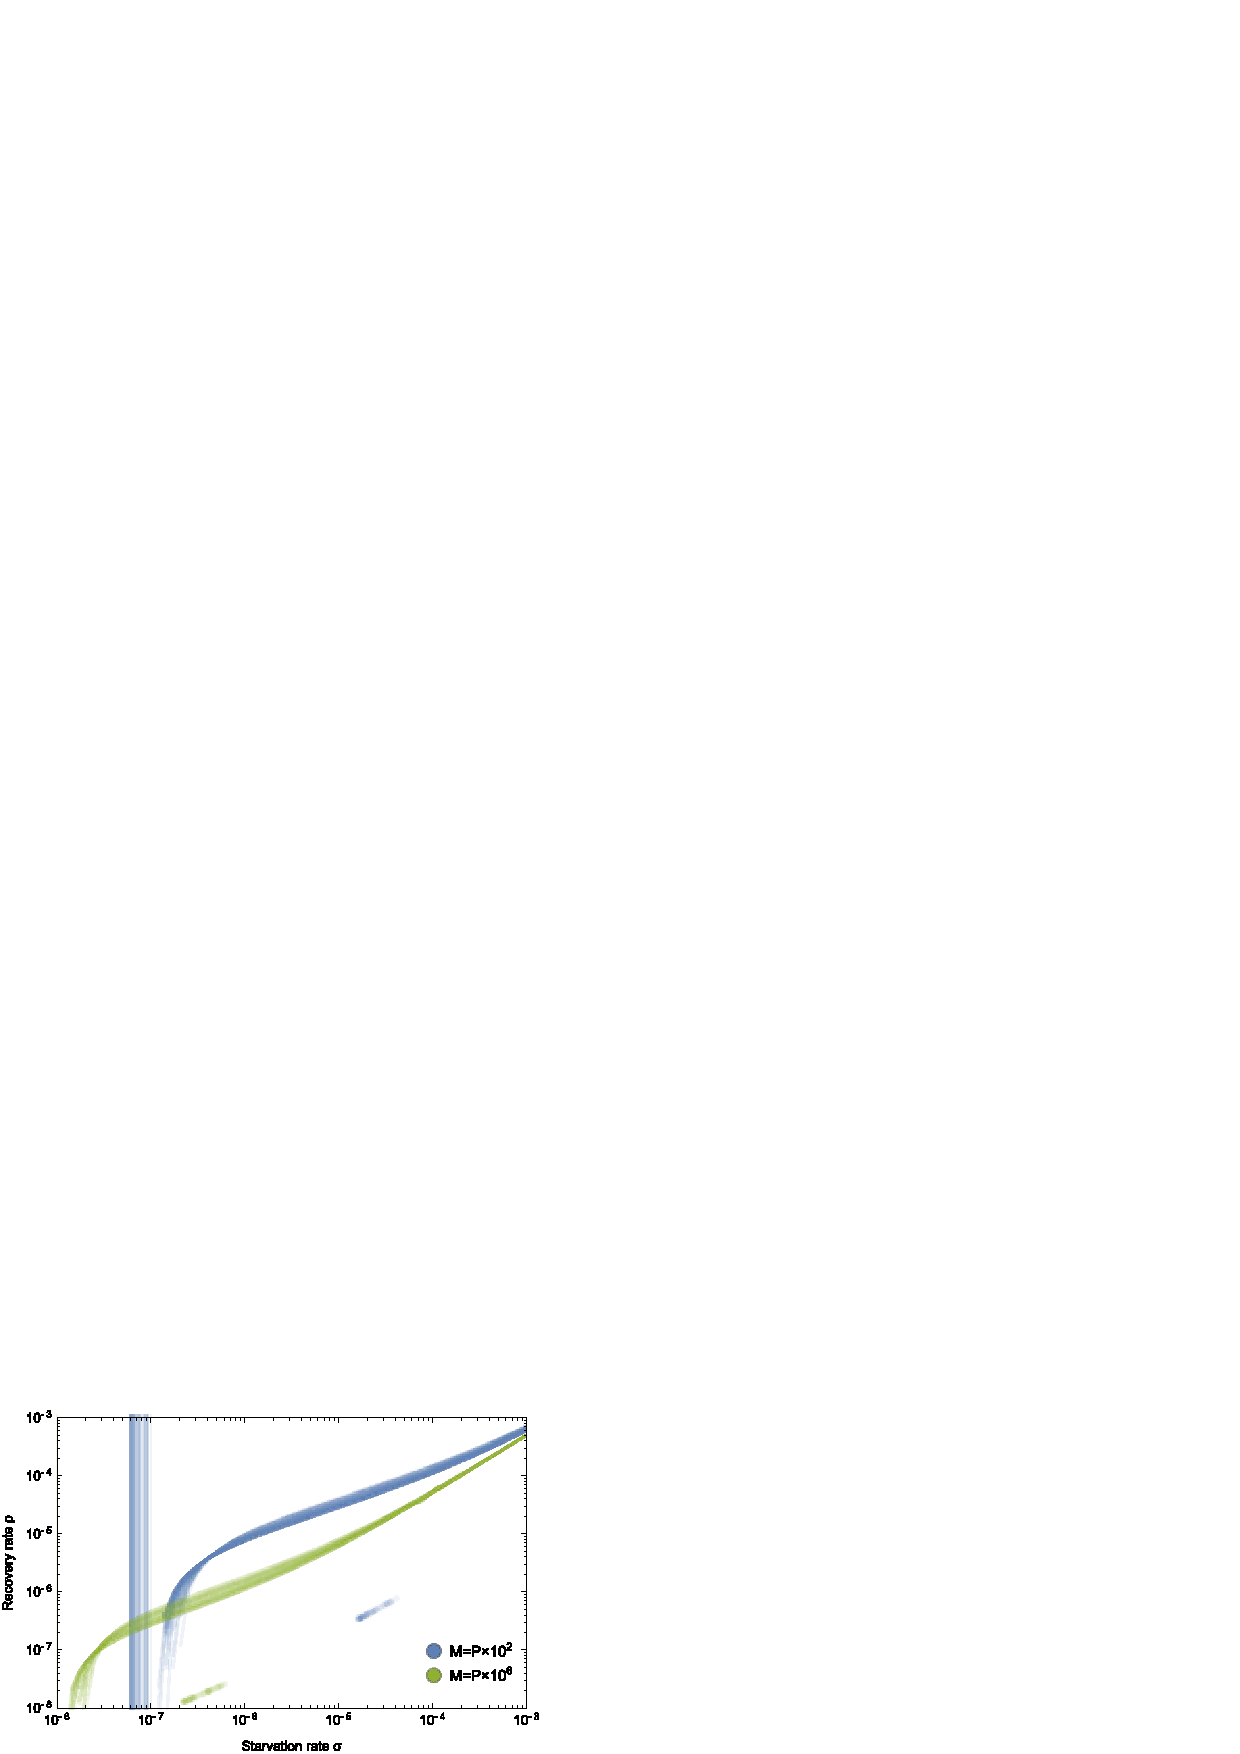
\includegraphics[width=0.8\textwidth]{fig_DataHopf.pdf}
 	\caption{
 	}
 	\label{DataHopf}
 \end{figure}
 
 
	\begin{figure}[h]
 	\centering
 	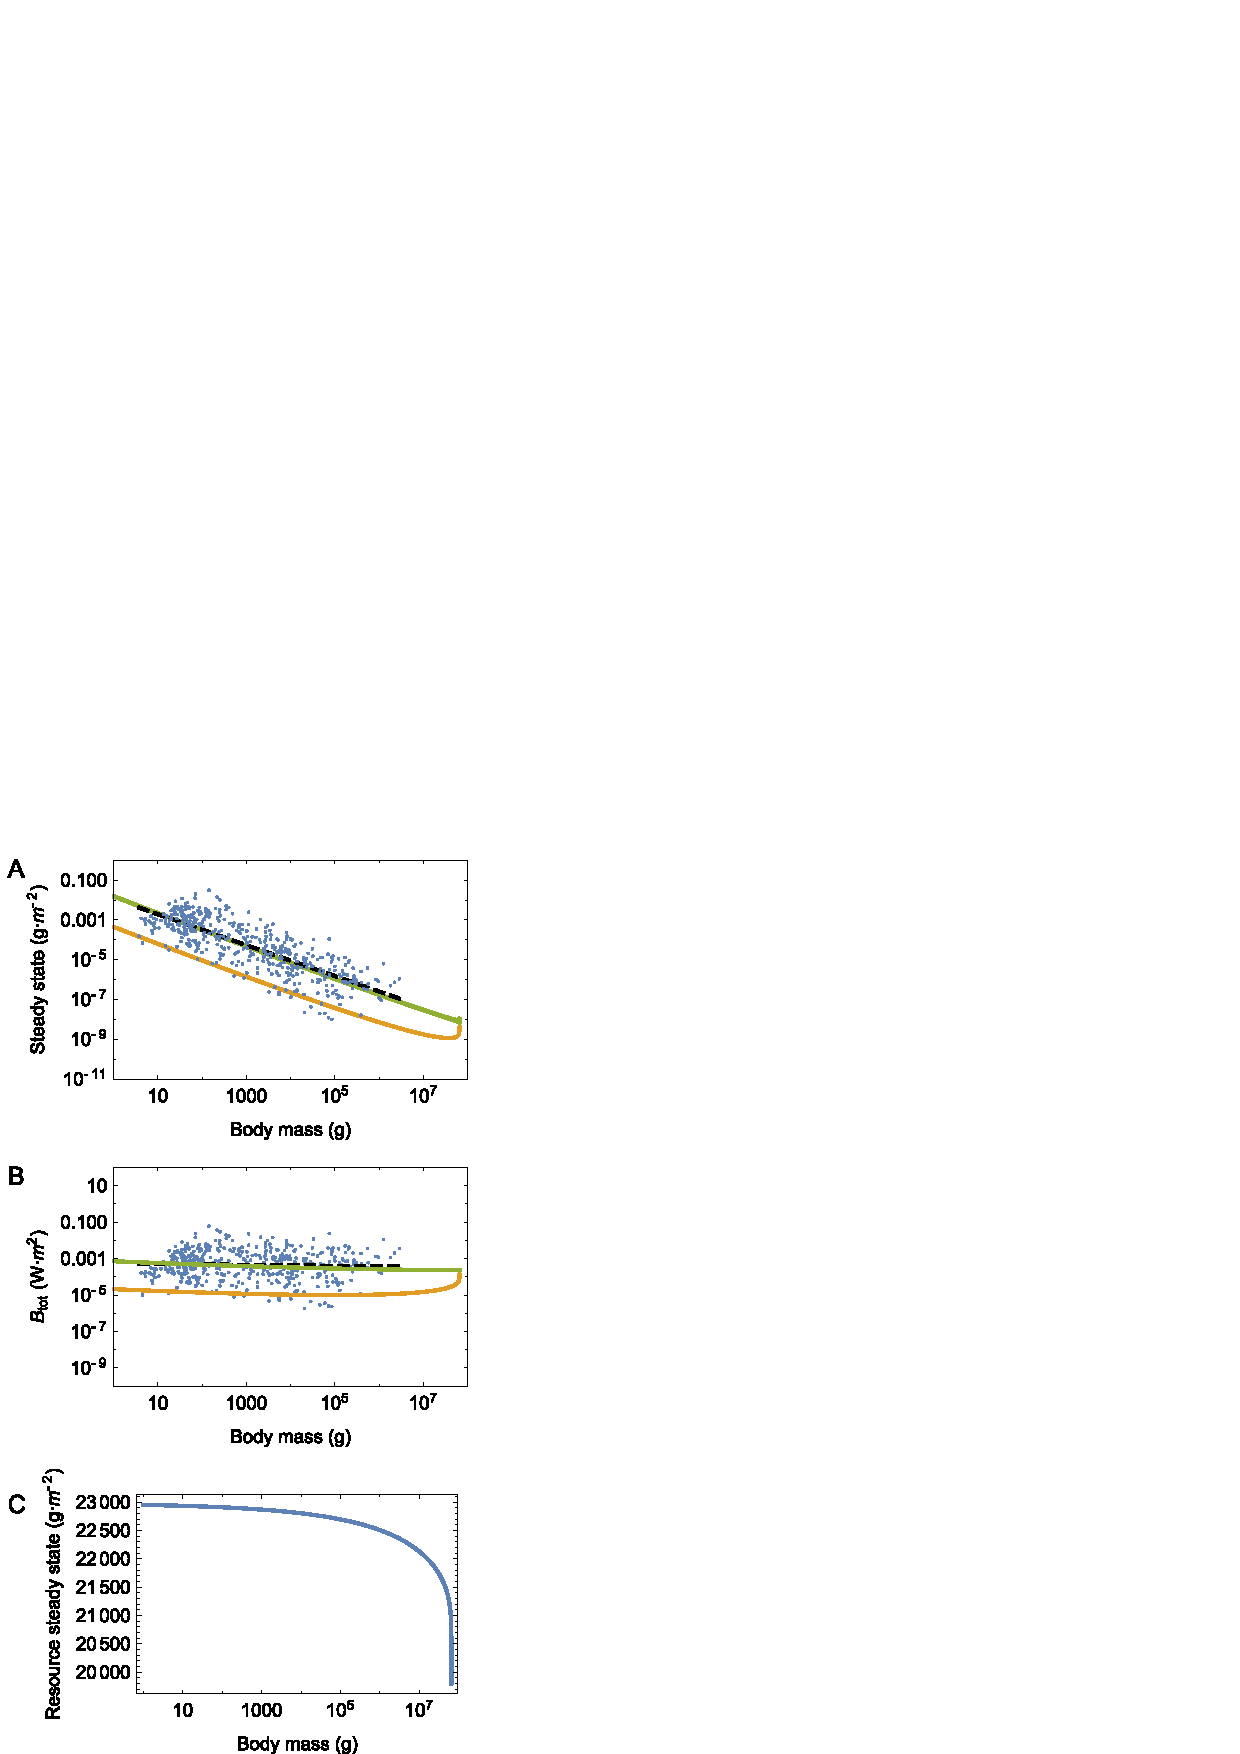
\includegraphics[width=0.5\textwidth]{fig_FPAllometric.pdf}
 	\caption{
 	}
 	\label{Asymp}
 \end{figure}
 
  \begin{figure}[h]
 	\centering
 	\includegraphics[width=0.8\textwidth]{fig_ExtinctionAllometric.pdf}
 	\caption{
 	}
 	\label{Ext}
 \end{figure}
 

 
%
%
% \begin{figure}[h]
% 	\centering
% 	\includegraphics[width=0.5\textwidth]{fig_resvuln.pdf}
% 	\caption{
% 	Probability that the resource value is less than threshold = 0.05
% 	}
% 	\label{SN}
% \end{figure}
%
%
%
% \begin{figure}[h]
% 	\centering
% 	\includegraphics[width=0.5\textwidth]{fig_Competition.pdf}
% 	\caption{
% 	Hopf bifurcation
% 	}
% 	\label{SN}
% \end{figure}

\clearpage

\section*{References}

\bibliographystyle{apalike} % for Science,
\bibliography{aa_starving}

%\end{flushleft}
\end{spacing}
\end{document}
